%%%%%%%%%%%%%%%%%%%%%%%%%%%%%%%%%%%%%%%%%
% Beamer Presentation
% LaTeX Template
% Version 1.0 (10/11/12)
%
% This template has been downloaded from:
% http://www.LaTeXTemplates.com
%
% License:
% CC BY-NC-SA 3.0 (http://creativecommons.org/licenses/by-nc-sa/3.0/)
%
%%%%%%%%%%%%%%%%%%%%%%%%%%%%%%%%%%%%%%%%%

%----------------------------------------------------------------------------------------
%	PACKAGES AND THEMES
%----------------------------------------------------------------------------------------

\documentclass{beamer}

\mode<presentation> {

% The Beamer class comes with a number of default slide themes
% which change the colors and layouts of slides. Below this is a list
% of all the themes, uncomment each in turn to see what they look like.

%\usetheme{default}
%\usetheme{AnnArbor}
%\usetheme{Antibes}
%\usetheme{Bergen}
%\usetheme{Berkeley}
%\usetheme{Berlin}
%\usetheme{Boadilla}
%\usetheme{CambridgeUS}
%\usetheme{Copenhagen}
%\usetheme{Darmstadt}
%\usetheme{Dresden}
%\usetheme{Frankfurt}
%\usetheme{Goettingen}
%\usetheme{Hannover}
%\usetheme{Ilmenau}
%\usetheme{JuanLesPins}
%\usetheme{Luebeck}
\usetheme{Madrid}
%\usetheme{Malmoe}
%\usetheme{Marburg}
%\usetheme{Montpellier}
%\usetheme{PaloAlto}
%\usetheme{Pittsburgh}
%\usetheme{Rochester}
%\usetheme{Singapore}
%\usetheme{Szeged}
%\usetheme{Warsaw}
\setbeamertemplate{navigation symbols}{}%remove navigation symbols
%\setbeamerfont{caption}{size=\scriptsize}

% As well as themes, the Beamer class has a number of color themes
% for any slide theme. Uncomment each of these in turn to see how it
% changes the colors of your current slide theme.

%\usecolortheme{albatross}
%\usecolortheme{beaver}
%\usecolortheme{beetle}
%\usecolortheme{crane}
%\usecolortheme{dolphin}
%\usecolortheme{dove}
%\usecolortheme{fly}
%\usecolortheme{lily}
%\usecolortheme{orchid}
%\usecolortheme{rose}
%\usecolortheme{seagull}
%\usecolortheme{seahorse}
%\usecolortheme{whale}
%\usecolortheme{wolverine}

%\setbeamertemplate{footline} % To remove the footer line in all slides uncomment this line
%\setbeamertemplate{footline}[page number] % To replace the footer line in all slides with a simple slide count uncomment this line

%\setbeamertemplate{navigation symbols}{} % To remove the navigation symbols from the bottom of all slides uncomment this line
\usefonttheme{serif}
}
\usepackage{transparent}
\usepackage{graphicx} % Allows including images
\usepackage{tikz}
\usepackage[duration=30,disablemarkdown]{pdfpc}
\usepackage[font=tiny, labelfont=bf]{caption}
\usepackage{subcaption}
\usepackage{booktabs} % Allows the use of \toprule, \midrule and \bottomrule in tables
\usepackage[%
    style=phys,%
    articletitle=false,biblabel=brackets,%
    chaptertitle=false,pageranges=false,%
    doi=false,maxnames=2,minnames=1,eprint=false%
  ]
{biblatex}
\addbibresource{library.bib}
\makeatletter
\renewcommand{\@makefnmark}{\makebox{\normalfont[\@thefnmark]}}
\renewcommand\@makefntext[1]{%
    {{\normalfont[\@thefnmark]}\enspace #1}
  }
\makeatother
%\renewcommand{\cite}[1]{[\footfullcite{#1}]}
\renewenvironment{equation}
    {
    \begin{equation*}
    }
    { 
    \end{equation*}
    }

%\renewenvironment{align}
    %{
    %\begin{align*}
    %}
    %{ 
    %\end{align*}
    %}
\renewcommand{\note}{\pdfpcnote}
%----------------------------------------------------------------------------------------
%	TITLE PAGE
%----------------------------------------------------------------------------------------

\title[Honors Presentation]{Topology of the $O(3)$ non-linear sigma model under the gradient flow} % The short title appears at the bottom of every slide, the full title is only on the title page

\author{Stuart Thomas} % Your name
\institute[W\&M] % Your institution as it will appear on the bottom of every slide, may be shorthand to save space
{
Christopher Monahan \\ % Your institution for the title page
\medskip
}
\date{May 3, 2021} % Date, can be changed to a custom date

\newcommand{\e}{\vec e}

\begin{document}
\setbeamerfont{footnote}{size=\tiny}
\begin{frame}
\titlepage % Print the title page as the first slide
\end{frame}

\begin{frame}
\titlepage % Print the title page as the first slide
\end{frame}


\begin{frame}
\frametitle{Quantum Field Theory}
   \centering
   \Huge particles $\Rightarrow$ fields
   \vspace{1cm}
\Large
   \begin{itemize}
       \item<2-> particle physics and condensed matter
       \item<3-> incorporates many-particle quantum mechanics and special relativity
       \item<4-> remarkably accurate \footfullcite{odom2006}

   \end{itemize}
   \note{What is a field? a mathematical object at every point of space and time.}
\end{frame}

\begin{frame}
    \frametitle{Path Integral Formulation}
    \Large\centering
``quantum principle of least action'' 
\begin{equation*}
    \label{eq:pathintegral}
    \langle \hat O \rangle = \frac{1}{Z} \int \mathcal{D}\phi \: \hat O [\phi]\; e^{iS[\phi]}
\end{equation*}
\note{Note vacuum}
\end{frame}

\begin{frame}
    \frametitle{Wick Rotation}
    \Large
    \begin{align*}
        t &\Rightarrow it \\
        \textrm{Minkowski Spacetime} &\Rightarrow \textrm{Euclidean Spacetime}
    \end{align*}
\vspace{0.1cm}
\hrule
\vspace{0.1cm}
    \onslide<2->{\begin{equation*}
        \langle \hat O \rangle = \frac{1}{Z} \int \mathcal{D}\phi \: \hat O [\phi]\; e^{iS[\phi]}
    \end{equation*}
    \[\Downarrow\]}
    \only<2>{\begin{equation*}
        \label{eq:pathintegraleuclidean}
        \langle \hat O \rangle = \frac{1}{Z} \int \mathcal{D}\phi \: \hat O [\phi]\; e^{-S_E[\phi]}
    \end{equation*}}
    \onslide<3>{\begin{equation*}
        \langle \hat O \rangle = \frac{1}{Z} \int \mathcal{D}\phi \: \hat O [\phi]\; \textcolor{red}{e^{-S_E[\phi]}}
    \end{equation*}}
\centering
\note{Downside: only possible for time-independent observables}
\end{frame}

\begin{frame}
\frametitle{$\phi^4$ model}
\begin{block}{Euclidean Action}
\begin{equation*}
    \label{eq:phi4 euclidean action}
    S_E[\phi] = \int d^2 x_E \left[\frac{1}{2}\left(\partial_t \phi\right)^2 + \frac{1}{2} \left(\partial_x \phi \right)^2 + \frac{1}{2} m_0^2 \phi^2 + \frac{\lambda}{4}\phi^4\right]
\end{equation*}
\end{block}
\begin{itemize}
    \item real scalar field
    \item describes a boson
    \item spontaneous symmetry breaking at $\lambda=0.5$, $m_0^2=-0.72$
\end{itemize}
\note{Check our simulation}
\end{frame}

\begin{frame}
\frametitle{Non-Linear $\sigma$ Model}
\begin{block}{Euclidean Action}
\begin{equation*}
    \label{eq:nlsm euclidean action}
    % S_E = \frac{\beta}{2} \int d^2x \; \partial^\mu \e \cdot \partial_\mu \e
    S_E = \frac{\beta}{2} \int d^2x \; \left[ \left(\partial_t \e\, \right)^2+ \left( \partial_x \e\,\right)^2 \right]
\end{equation*}
\end{block}
\begin{itemize}
    \item<1-> $O(3)$ non-linear sigma model (NLSM) in 1+1 dimensions
    \item<2-> $\e$ is 3-component vector constrained by $|\e\,|=1$
    \item<3-> Applications
        \begin{itemize}
            \item Prototypical model for strong nuclear force
            \item Models Heisenberg ferromagnets
            \item Applications to string theory
        \end{itemize}
    \item<4-> Merits 
        \begin{itemize}
            \item mass gap
            \item asymptotic freedom
        \end{itemize}
\end{itemize}
\end{frame}

\begin{frame}
    \frametitle{Topology of 1+1 $O(3)$ NLSM}
    \begin{columns}

    \begin{column}{0.5\textwidth}
    \begin{enumerate}
        \item<1-> Envision spacetime as a sphere
        \item<2-> The NLSM field $\e$ becomes mapping between Riemann spheres ($S^2 \rightarrow S^2$).
        \item<3-> Associates every configuration with topological charge $Q$
        \item<4-> Topology is important to cosmology\footnotemark[2]\ and fault-tolerant quantum computing\footnotemark[3]. 
    \end{enumerate}
    \end{column}
    \begin{column}{0.5\textwidth}
        \begin{figure}
            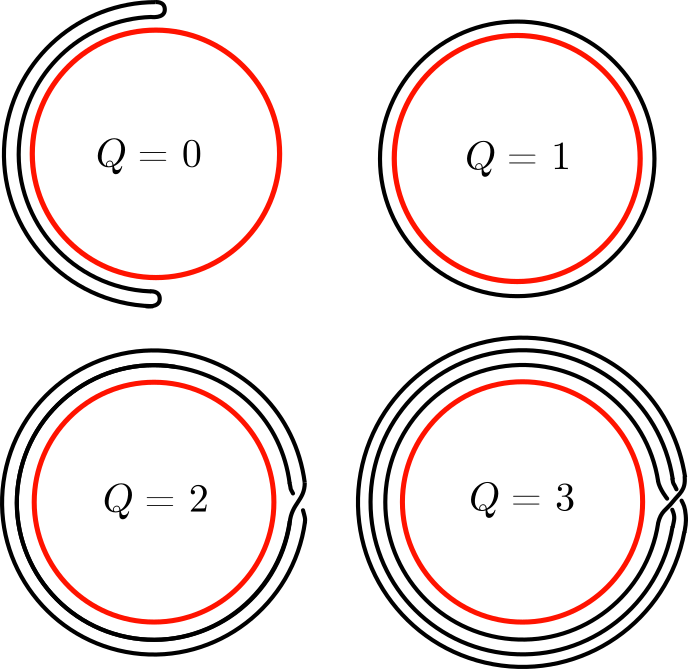
\includegraphics[width=0.3\paperwidth]{imgs/homotopy.png}
            \caption{\label{fig:homotopy} Homotopy group of $S^1\rightarrow S^1$}
        \end{figure}
    \end{column}
    \end{columns}
    \footnotetext[2]{\fullcite{goddard1986}}
    \footnotetext[3]{\fullcite{kitaev1997}}
\note{Many people are not familiar with topology \\%
    1. Since the Lagrangian must disappear at infinity, the field must be uniform for all points as x -> infty. \\%
    2. We can classify every mapping with an integer. Use ball and balloon metaphor}
\end{frame}

\begin{frame}
    \frametitle{Non-trivial NLSM}
    \begin{equation*}
        S[\e\,] \rightarrow S[\e\,] - i \theta Q[\e\,].
    \end{equation*}
    Nonzero $\theta$ implies nonzero $\langle Q \rangle$.
\end{frame}

\begin{frame}
    \frametitle{Topological Susceptibility}
    \centering
    Proportional to variance of topological charge
    \begin{equation}
        \chi_t \equiv \frac{\langle Q^2 \rangle - \langle Q \rangle^2}{L^2}
    \end{equation}
    \onslide<2->{
        \vfill
        \hrule
        \vfill
        \begin{columns}
            \begin{column}{0.5\textwidth}
                \centering
            In trivial NLSM:
            \begin{equation}
                \chi_t = \frac{\langle Q^2 \rangle}{L^2}
            \end{equation}
            \end{column}
        
        %\only<3->{
            \begin{column}{0.5\textwidth}
                \centering
            In nontrivial NLSM:
            \begin{equation}
                \chi_t \propto \frac{\partial\langle Q \rangle}{\partial \theta} 
            \end{equation}
            \end{column}
        %}
        \end{columns}
    }
    \onslide<3->\begin{block}{Main Problem}
        Topological stability predicts $\chi_t=0$, but $\chi_t$ diverges in numerical results \footfullcite{berg1981}.
    \end{block}
\end{frame}

\begin{frame}
\frametitle{The Gradient Flow}
\begin{itemize}
    \item<1-> Successful in removing $\chi_t$ divergence in QCD (model of the strong nuclear force).
    \item<2-> Reduces high-momentum modes
    \item<3-> Introduces a new dimension, $\tau$, called the ``flow time,'' which pushes fields towards action minima 
    \item<4-> In the $\phi^4$ model
    \begin{equation*}
        \frac{\partial \rho(\tau, x)}{\partial \tau} = \partial^2 \rho(\tau,x)
    \end{equation*}
    with the boundary condition $\rho(0, x)=\phi(x)$.

\end{itemize}
\onslide<4->\begin{figure}[h]
  \centering
      \begin{subfigure}[b]{0.2\textwidth}\centering
        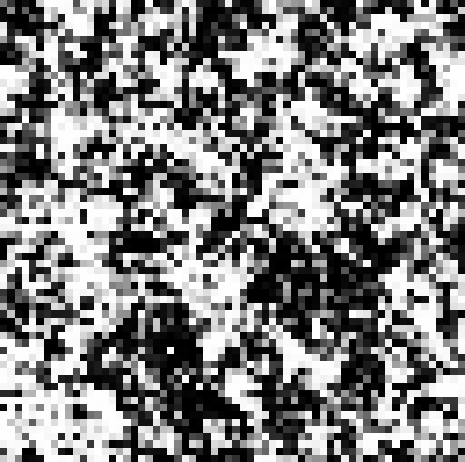
\includegraphics[width=0.9\textwidth]{imgs/gf0.png}
        \caption{$\tau=0$}
      \end{subfigure}%
      \begin{subfigure}[b]{0.2\textwidth}\centering
        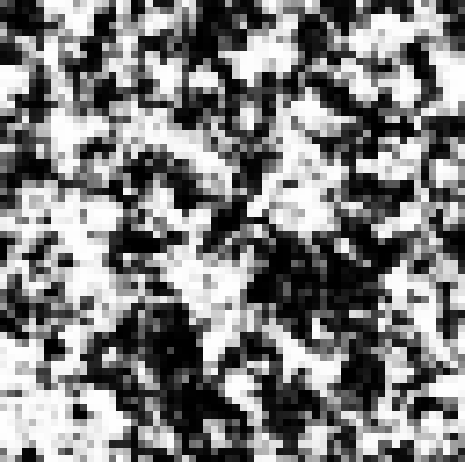
\includegraphics[width=0.9\textwidth]{imgs/gf1.png}
        \caption{$\tau=0.001$}
      \end{subfigure}%
      \begin{subfigure}[b]{0.2\textwidth}\centering
        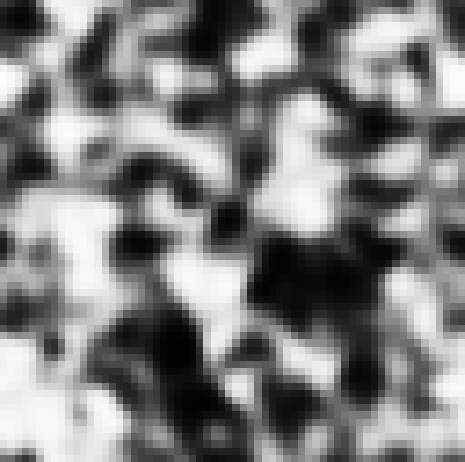
\includegraphics[width=0.9\textwidth]{imgs/gf2.png}
        \caption{$\tau=0.01$}
      \end{subfigure}%
      \begin{subfigure}[b]{0.2\textwidth}\centering
        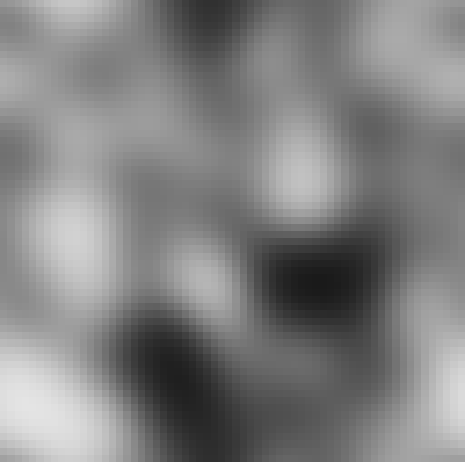
\includegraphics[width=0.9\textwidth]{imgs/gf3.png}
        \caption{$\tau=0.1$}
      \end{subfigure}%
      \caption{\label{fig:flow} Effect of flow time evolution on a random lattice in the symmetric phase. White represents positive values of $\phi$ while black represents negative.}
\end{figure}
\note{Effect of flow time evolution on a random lattice in the symmetric phase. Red and blue indicate positive and negative values of the field in 2D spacetime.}
\end{frame}

\begin{frame}
   \centering
   \begin{block}{Research Question}
       Can the gradient flow remove the topological susceptibility divergence in the NLSM?
   \end{block}
\end{frame}

\begin{frame}
\frametitle{Methods}
\begin{enumerate}
    \item Construct Monte Carlo simulation following Euclidean path integral formalism
    \item Apply gradient flow to configurations
    \item Measure topological susceptibility
\end{enumerate}
\end{frame}

\begin{frame}
    \frametitle{Fields on the Lattice}
    \begin{align*}
        x & \rightarrow ia \hat{t} + j a \hat{x} \\
        \int dtdx &\rightarrow a^2 \sum_i
    \end{align*}

    where $a$ is the lattice spacing. 

    \vspace{0.3cm}\hrule\vspace{0.3cm}

    Periodic boundary conditions:
    \begin{equation}
        \phi\left(x_{i+L,j}\right) = \phi\left(x_{i,j+L}\right) = \phi\left(x_{i,j}\right)
    \end{equation}
\end{frame}

\begin{frame}
    \frametitle{Markov chain Monte Carlo}
    \onslide<1-> Due to Boltzmann factor $e^{-S}$, we need only consider configurations near action minima.
    \begin{itemize}
        \item<2-> Starting at configuration $\phi_a$, we transition to configuration $\phi_b$ with probability 
        \[P(\phi_a \rightarrow \phi_b).\]
    \end{itemize}
    \note{Mention infinite path integral}
\end{frame}

\begin{frame}
    \frametitle{Metropolis Algorithm}
    Changes a single site randomly
    \begin{equation}
        P(\phi_a\rightarrow\phi_b) = \begin{cases} 
            e^{S[\phi_a] - S[\phi_b]} & S[\phi_b] > S[\phi_a] \\
            1 & \mathrm{otherwise} \\
       \end{cases}
    \end{equation}
    Performing this process on every site forms a ``sweep''
\end{frame}

\begin{frame}
    \frametitle{Wolff Cluster Algorithm}
    Grows one cluster probabilistically, flips sign~\footfullcite{wolff1989}
    \begin{figure}[h]
      \centering
          \begin{subfigure}[b]{0.5\textwidth}\centering
            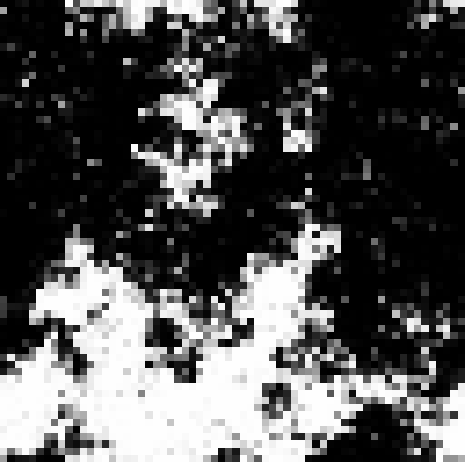
\includegraphics[width=0.6\textwidth]{imgs/wolffa.png}
            \caption{before cluster flip}
          \end{subfigure}%
          \hfill
          \begin{subfigure}[b]{0.5\textwidth}\centering
            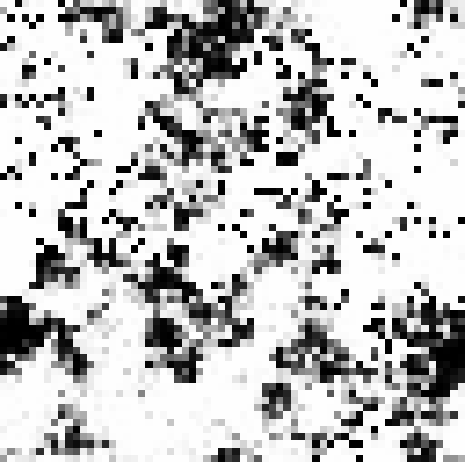
\includegraphics[width=0.6\textwidth]{imgs/wolffb.png}
            \caption{after cluster flip}
          \end{subfigure}
          \hfill
          %\caption{\label{fig:wolff} An example of the Wolff cluster algorithm in the $\phi^4$ model. White represents positive values of $\phi$ while black represents negative. $\lambda=0.5$, $m_0^2=-0.9$.}
    \end{figure}
    \note{What about NLSM?}
\end{frame}

\begin{frame}
    \frametitle{Thermalization}

    How do we start the Markov chain?
    \begin{columns}

        \begin{column}{0.5\textwidth}
            \begin{figure}[h]
              \centering
                  \begin{subfigure}[b]{0.8\textwidth}\centering
                    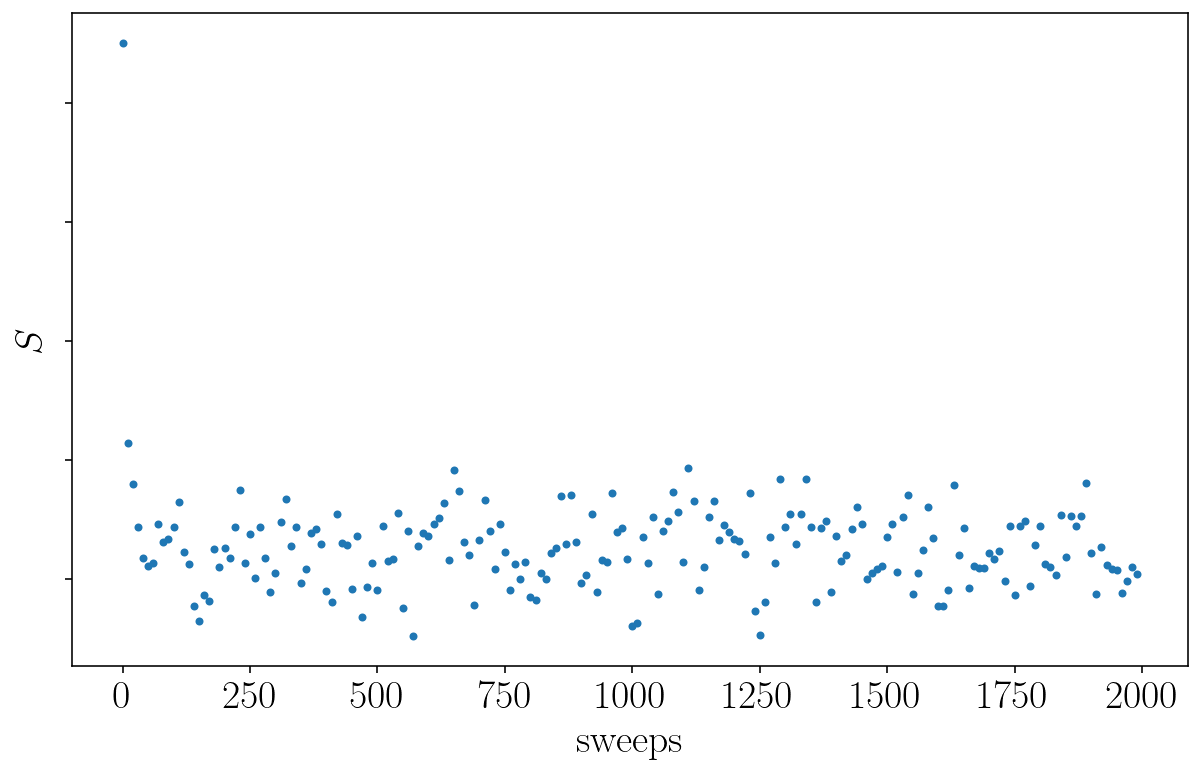
\includegraphics[width=\textwidth]{imgs/therm24.png}
                    \caption{$L=24$}
                  \end{subfigure}
                  \begin{subfigure}[b]{0.8\textwidth}\centering
                    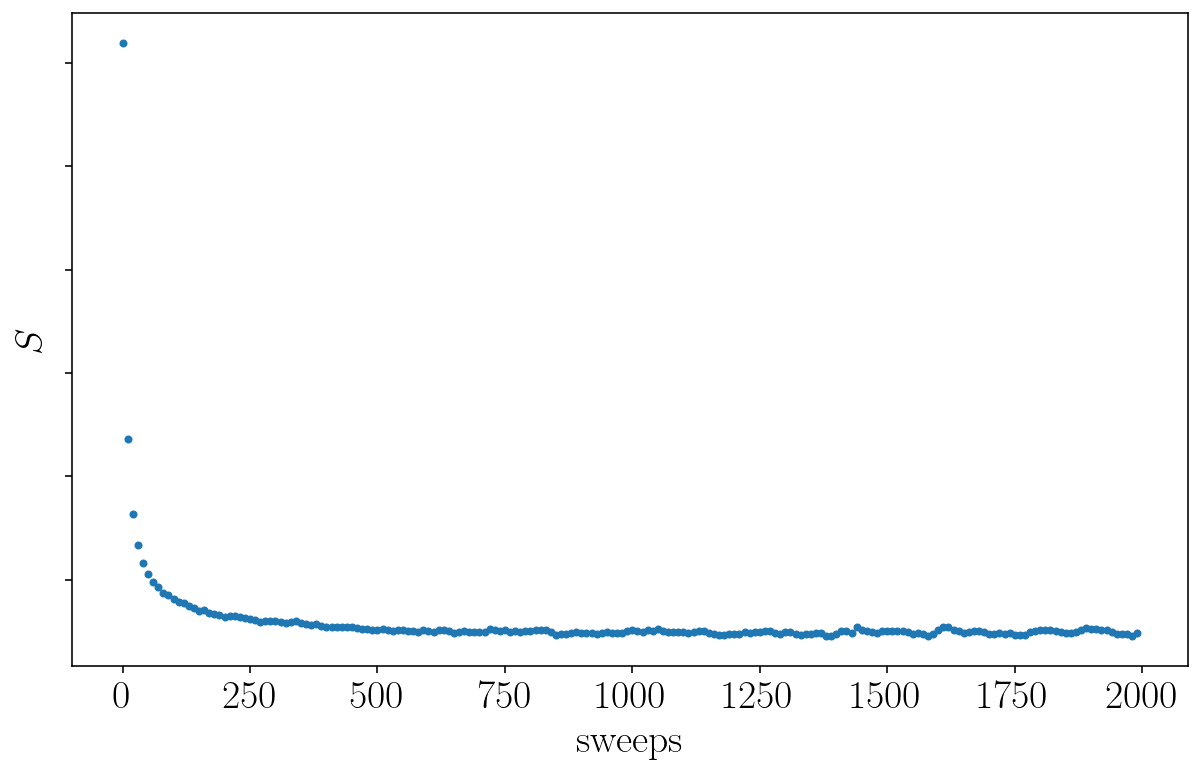
\includegraphics[width=\textwidth]{imgs/therm404.png}
                    \caption{$L=404$}
                  \end{subfigure}
                  \hfill
            \end{figure}
        \end{column}
        \begin{column}{0.5\textwidth}
            \onslide<2->{
            \begin{figure}[h]
              \centering
                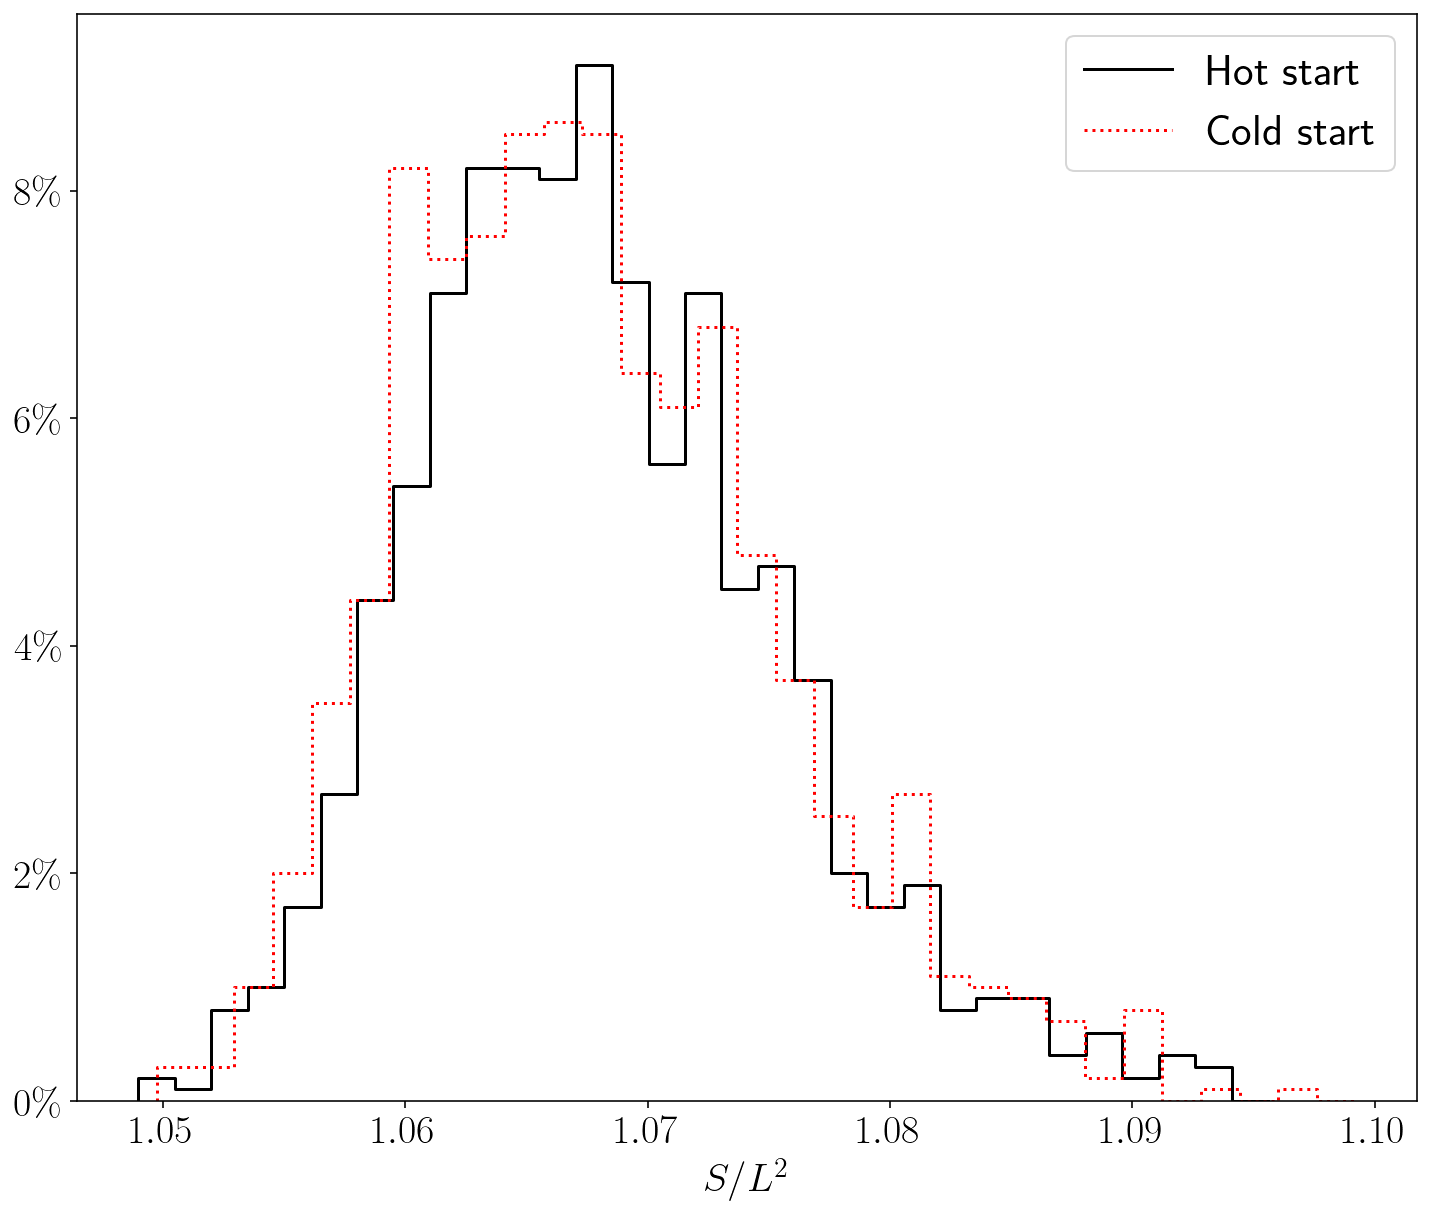
\includegraphics[width=0.9\textwidth]{imgs/coldstart.png}
                \caption{Action histogram comparing hot vs. cold start after 1000 sweep thermalization}
            \end{figure}
            }
        \end{column}
    \end{columns}
      \note{Plots of the action as a function of Monte Carlo time, starting with a random NLSM lattice. \\ Histogram of lattice-averaged actions $S/L^2$ with hot and cold starts. 1,000 sweep thermalization in $L=404$ lattice, 1,000 measurements taken every 50 sweeps.}
\end{frame}

\begin{frame}
    \frametitle{Autocorrelation}
    How many sweeps per measurement?
    \begin{figure}[h]
      \centering
          \begin{subfigure}[b]{0.5\textwidth}\centering
            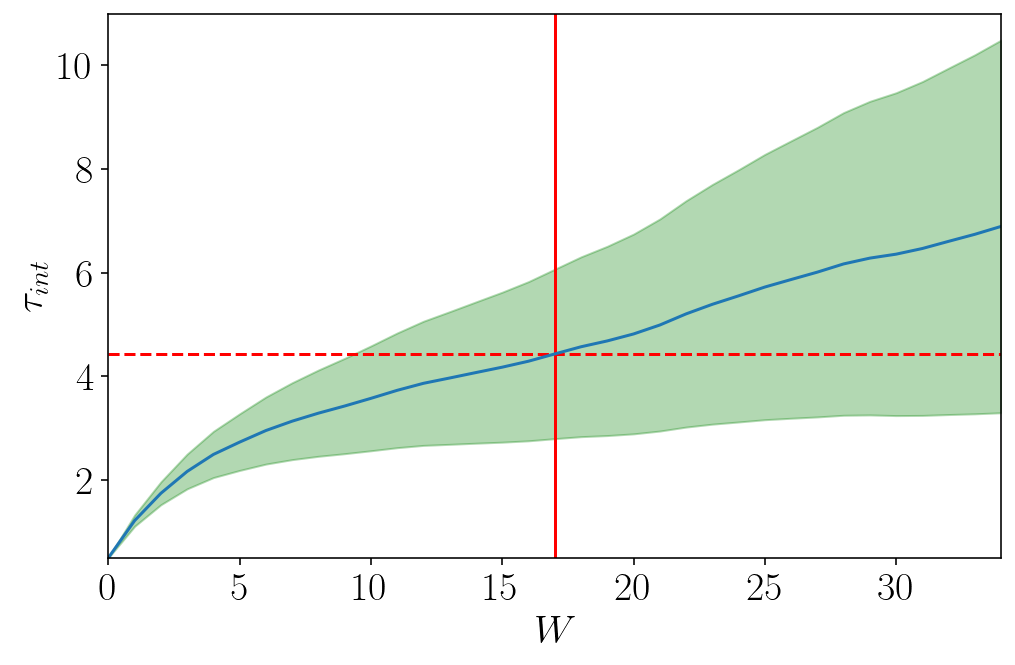
\includegraphics[width=0.9\textwidth]{imgs/tauint24.png}
            \caption{$L=24$, $\tau_{int}=4.43$}
          \end{subfigure}%
          \hfill
          \begin{subfigure}[b]{0.5\textwidth}\centering
            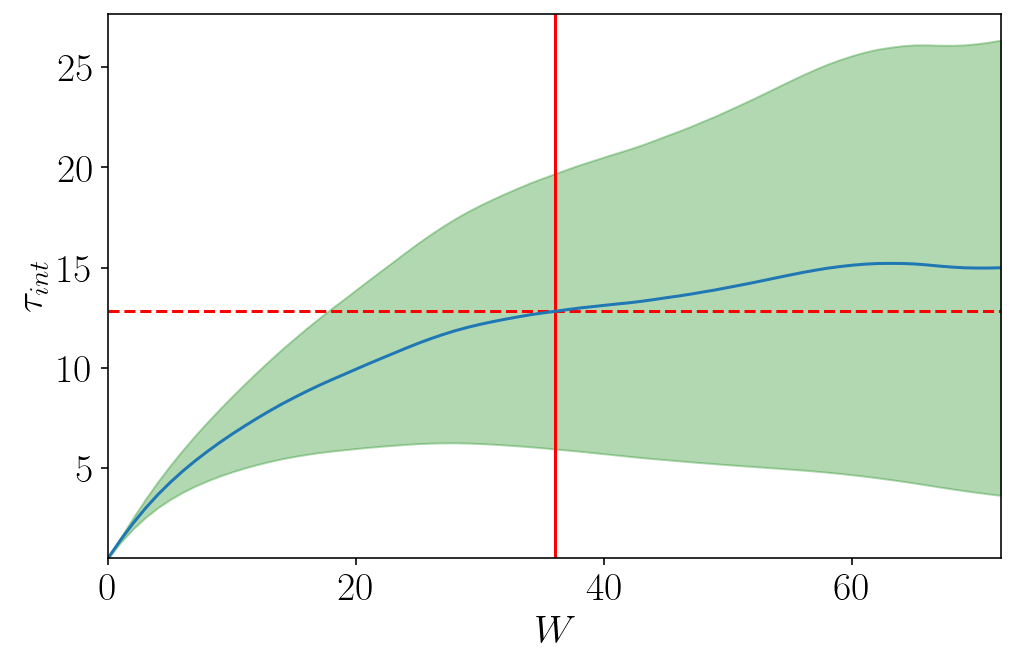
\includegraphics[width=0.9\textwidth]{imgs/tauint404.png}
            \caption{$L=404$, $\tau_{int}=12.81$}
          \end{subfigure}
          \hfill
          \caption{\label{fig:tauint} Plots of automatic windowing\footfullcite{wolff2007} procedure used to calculate $\tau_{int}$ for the NLSM model. $W$ is summation window size.}
    \end{figure}
    Therefore, we measure every 50 sweeps with a Wolff cluster step every 5 sweeps.
\end{frame}

\begin{frame}
    \frametitle{Topological Charge on the Lattice}
    Following Berg \& L\"usher~\footfullcite{berg1981}, define topological charge density $q(x^*)$ for each plaquette $x^*$ such that
    \begin{equation}
        Q = \sum_{x^*} q(x^*)
    \end{equation}
    \begin{figure}[h]
    \begin{subfigure}[b]{0.4\paperwidth}
    \centering
    \begin{tikzpicture}[scale=0.4, every node/.style={scale=0.7}]
        \draw[step=4cm,gray,thin] (-1,-1) grid (5,5);
        \draw[dotted] (0,0) -- (4,4);
        \draw[thick](0,0) node[circle,fill,inner sep=0pt, minimum size=0.3cm]{} node[anchor=north west] {$x_1$} -- 
                    (0,4) node[circle,fill,inner sep=0pt, minimum size=0.3cm]{} node[anchor=north west] {$x_2$} -- 
                    (4,4) node[circle,fill,inner sep=0pt, minimum size=0.3cm]{} node[anchor=north west] {$x_3$} -- 
                    (4,0) node[circle,fill,inner sep=0pt, minimum size=0.3cm]{} node[anchor=north west] {$x_4$} -- cycle ;
                    \draw[] (2,2) node[circle,fill,inner sep=0pt, minimum size=0.3cm]{} node[anchor=north east]{$x^*$};


        \draw[-stealth] (0.2,1) -- (0.2,3);
        \draw[-stealth] (1,3.8) -- (3,3.8);
        \draw[-stealth] (3,3.5) -- (1,1.5);

        \draw[-stealth] (1,0.5) -- (3,2.5);
        \draw[-stealth] (3.8,3) -- (3.8,1);
        \draw[-stealth] (3,0.2) -- (1,0.2);
    \end{tikzpicture}
    \caption{a plaquette}
    %\caption{\label{fig:plaquette} Visualization of plaquette $x^*$. The dotted line separates the plaquette into two signed areas which are used to define the topological charge density $q(x^*)$. Arrows represent order of signed area.}
    \end{subfigure} %
    \begin{subfigure}[b]{0.4\paperwidth}
    \centering
    \begin{tikzpicture}[scale=0.5, every node/.style={scale=0.7}]
        \pgfdeclarelayer{nodelayer}
        \pgfdeclarelayer{edgelayer}
        \pgfdeclareradialshading{sphere4}{\pgfpoint{-0.2cm}{0.5cm}}% 
            {rgb(0cm)=(1,1,1);
            rgb(1cm)=(0.5,0.5,0.5); rgb(1.05cm)=(1,1,1)}
            %rgb(0.7cm)=(0.1,0.1,0.1); rgb(1cm)=(0.5,0.05,0); rgb(1.05cm)=(1,1,1)}
        \pgfsetlayers{nodelayer,edgelayer}
        \tikzstyle{label}=[fill=none, draw=none, shape=circle]
        \tikzstyle{point}=[inner sep=0pt, minimum size=0.2cm,fill=black, draw, shape=circle]
        %\tikzstyle{interior line}=[{Stealth[scale=1.5]}-,dotted,thick]
        \tikzstyle{interior line}=[dotted,thick]

        \tikzstyle{triangle}=[thick]
        \tikzstyle{arrow}=[->, thick]
        \begin{pgfonlayer}{nodelayer}
            \node [style=point] (4) at (0.5, 2.5) {};
            \node [style=point] (5) at (0.55, 0.625) {};
            \node [style=point] (6) at (2.25, 0.75) {};
            \node (7) at (0, 0) {};
            \node (8) at (1.25, 1.375) {};
            \node (9) at (2.425, 2.525) {};
        \end{pgfonlayer}
        \begin{pgfonlayer}{edgelayer}
            \draw (0,0) circle (3cm);
            %\shade[inner color=white,outer color=lightgray] (0,0) circle (3cm);
            \shade[shading=sphere4] (0,0) circle (3cm);
            \draw [bend left=15,style=triangle] (4.center) to (6.center);
            \draw [bend left=355,style=triangle] (6.center) to (5.center);
            \draw [bend right=5,style=triangle] (5.center) to (4.center);
            \draw [style=interior line] (4.center) to (7.center);
            \draw [style=interior line] (5.center) to (7.center);
            \draw [style=interior line] (6.center) to (7.center);
            \draw [fill=gray!80] (4.center) to [bend left=15] (6.center) to [bend left=355] (5.center) to [bend right=5] cycle;

            %\draw [style=arrow] (8.center) to (9.center);

            \node [style=label, anchor=north] at (2.25, 0.75) {\small $\e(x_1)$};
            \node [style=label, anchor=north] at (0.55, 0.625) {\small $\e(x_2)$};
            \node [style=label, anchor=east] at (0.5, 2.5) {\small $\e(x_3)$};
            \node [style=point] at (4){};
            \node [style=point] at (5){};
            \node [style=point] at (6){};

            \node [style=label] at (8) {\small $A$};
        \end{pgfonlayer}
    \end{tikzpicture}
    \caption{signed area of triangle}
    \end{subfigure}
    \end{figure}
    \begin{equation}
        q(x^*) = \frac{1}{4\pi} \bigg[A\Big(\e(x_1), \e(x_2), \e(x_3)\Big) + A\Big(\e(x_1), \e(x_3), \e(x_4)\Big) \bigg].
    \end{equation}
\end{frame}

\begin{frame}
    \frametitle{Topological Charge Measurement}
    \begin{figure}[h]
    \centering
      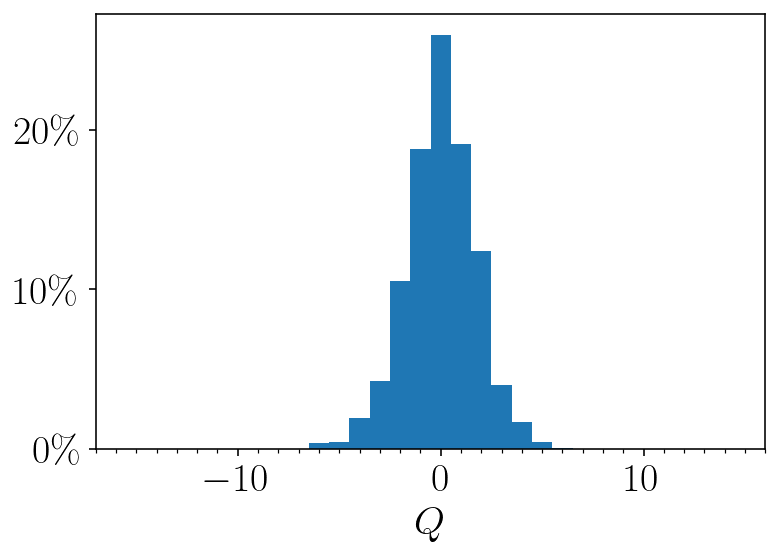
\includegraphics[width=0.6\textwidth]{imgs/hist.png}
      \caption{Histogram of topological charge values $Q$ for trivial NLSM. $L=404$, 10,000 measurements.}
\end{figure}
      \note{Histogram of topological charge values $Q$ for trivial NLSM. $L=404$, 10,000 measurements, measurements very 50 sweeps, 1,000 sweep thermalization, $\tau=0$}
\end{frame}


\begin{frame}
    \frametitle{Gradient flow on NLSM}
    We solve the Gradient Flow numerically using
    \begin{itemize}
        \item fourth-order Runge Kutta
        \item adaptive step size
    \end{itemize}
\end{frame}

\begin{frame}
    \frametitle{$\phi^4$ results}
    \begin{figure}[h!]
        \centering
          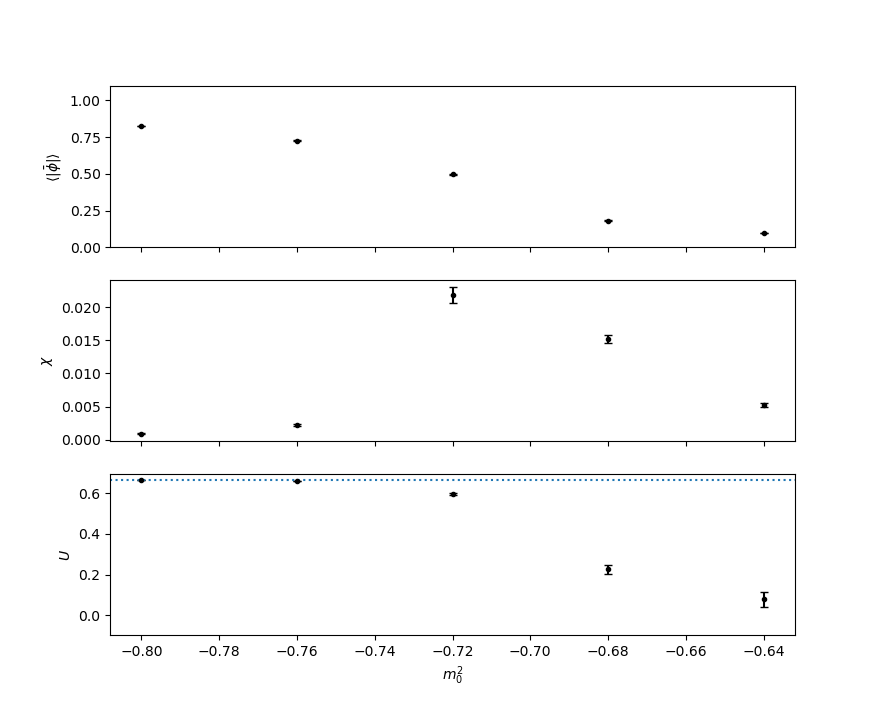
\includegraphics[width=0.7\textwidth]{imgs/phi4.png}
          \caption{\label{fig:phi4} The lattice average $|\langle\bar\phi\rangle|$, the magnetic susceptibility $\chi_m$, the Binder cumulant $U\:$ ~\footfullcite{binder1981} and the bimodality $B$ plotted as functions of $m_0^2$. $L=64$, $\lambda=0.5$. 1000 measurements}
    \end{figure}
    \note{First mention broken and symmetric phases}
\end{frame}

\begin{frame}
    \frametitle{Comparison with Berg \& L\"uscher}
    \begin{figure}[h!]
        \centering
          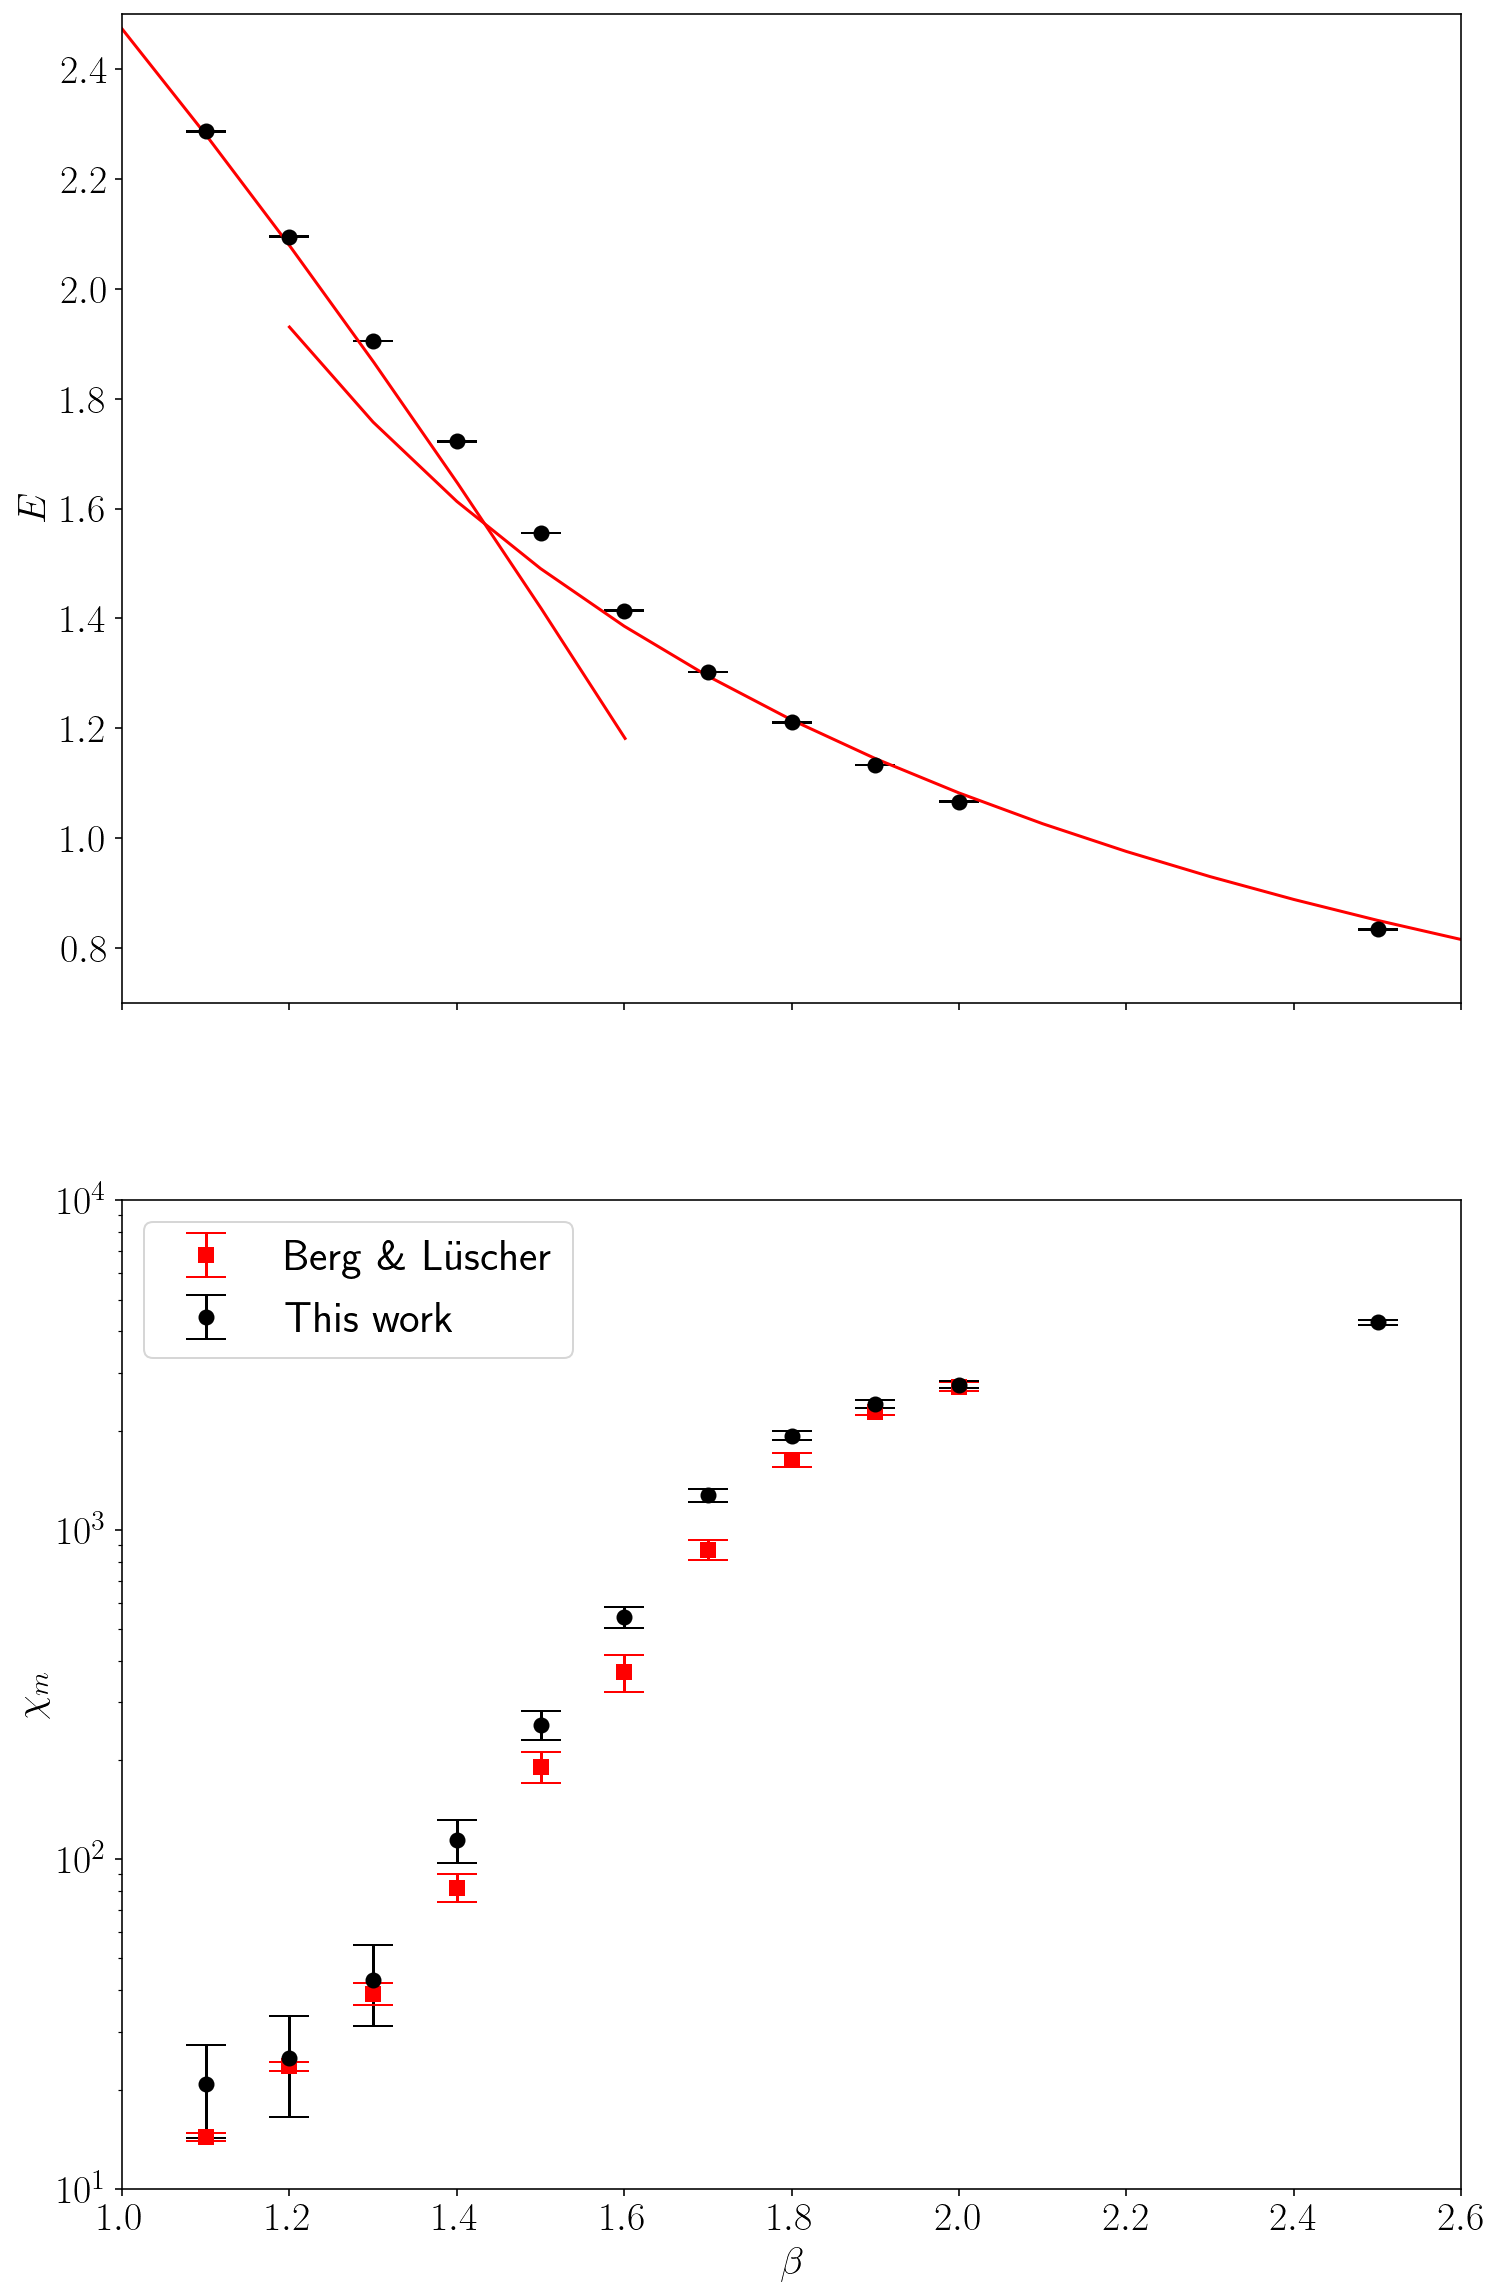
\includegraphics[width=0.9\textwidth]{imgs/internal_energy.png}
          \caption{\label{fig:bergluscher}Comparison with~\footfullcite{berg1981}, $L=100$, 1000 measurements.}
    \end{figure}
\end{frame}



\begin{frame}
    \frametitle{Topological Susceptibility in Flow Time}
    \begin{figure}[h!]
        \centering
          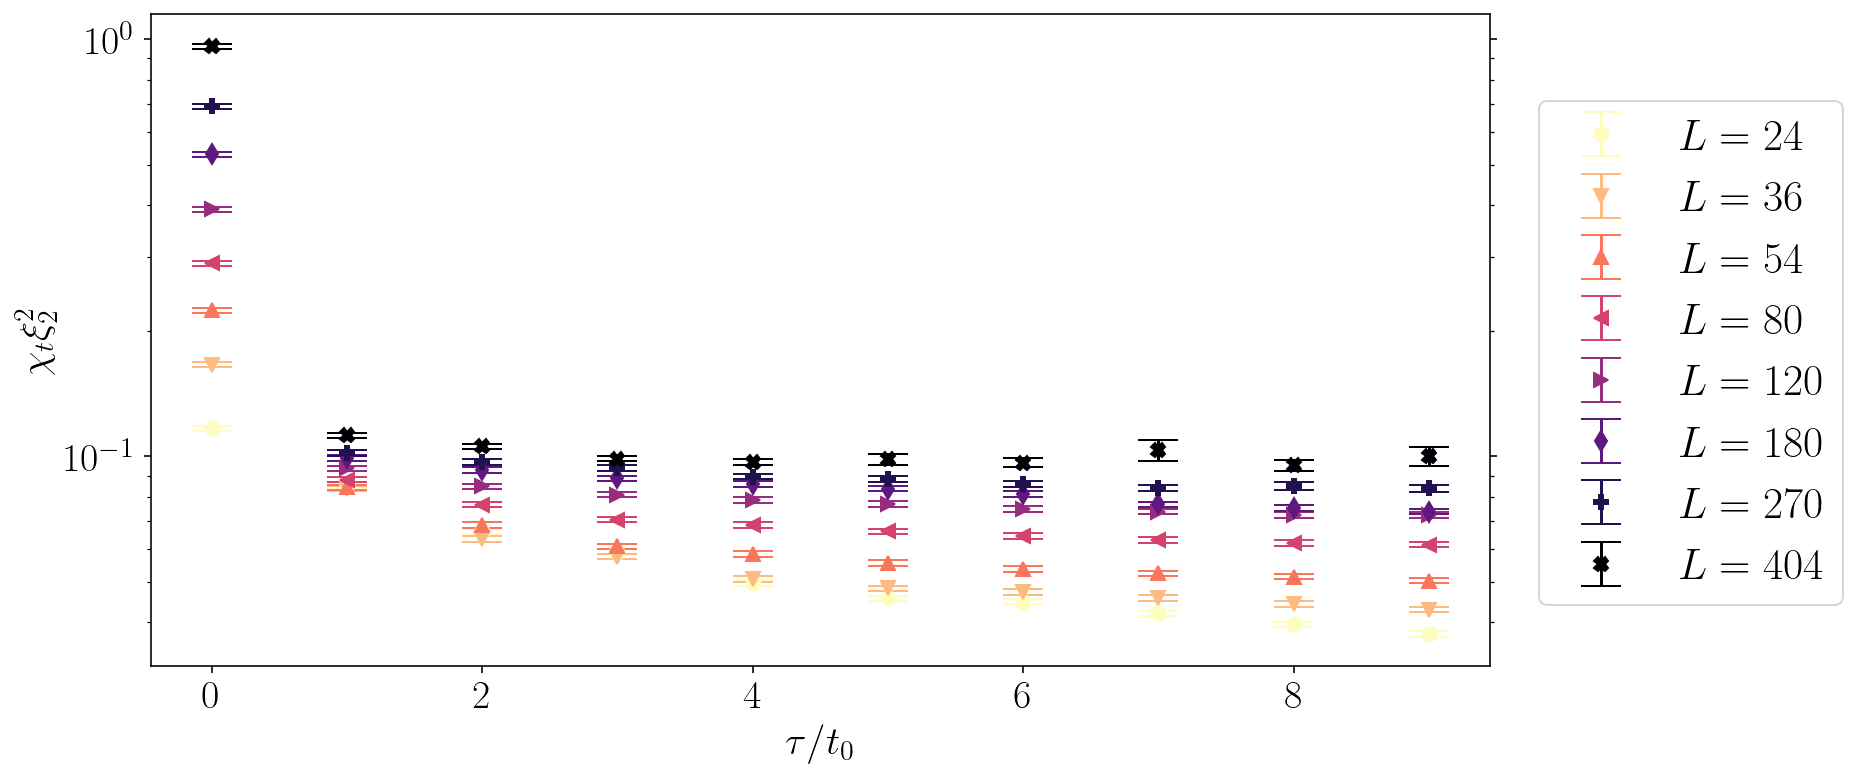
\includegraphics[width=\textwidth]{imgs/bietenholz.png}
          \caption{\label{fig:bietenholz} $\chi_t \xi_2^2$ as a  function of flow time $\tau$. Simulation run with 10,000 measurements }
    \end{figure}
\end{frame}


\begin{frame}
    \frametitle{$\chi_t$ Divergence}
    \begin{figure}[h!]
        \begin{center}
          \begin{subfigure}[b]{0.45\paperwidth}

              \centering
              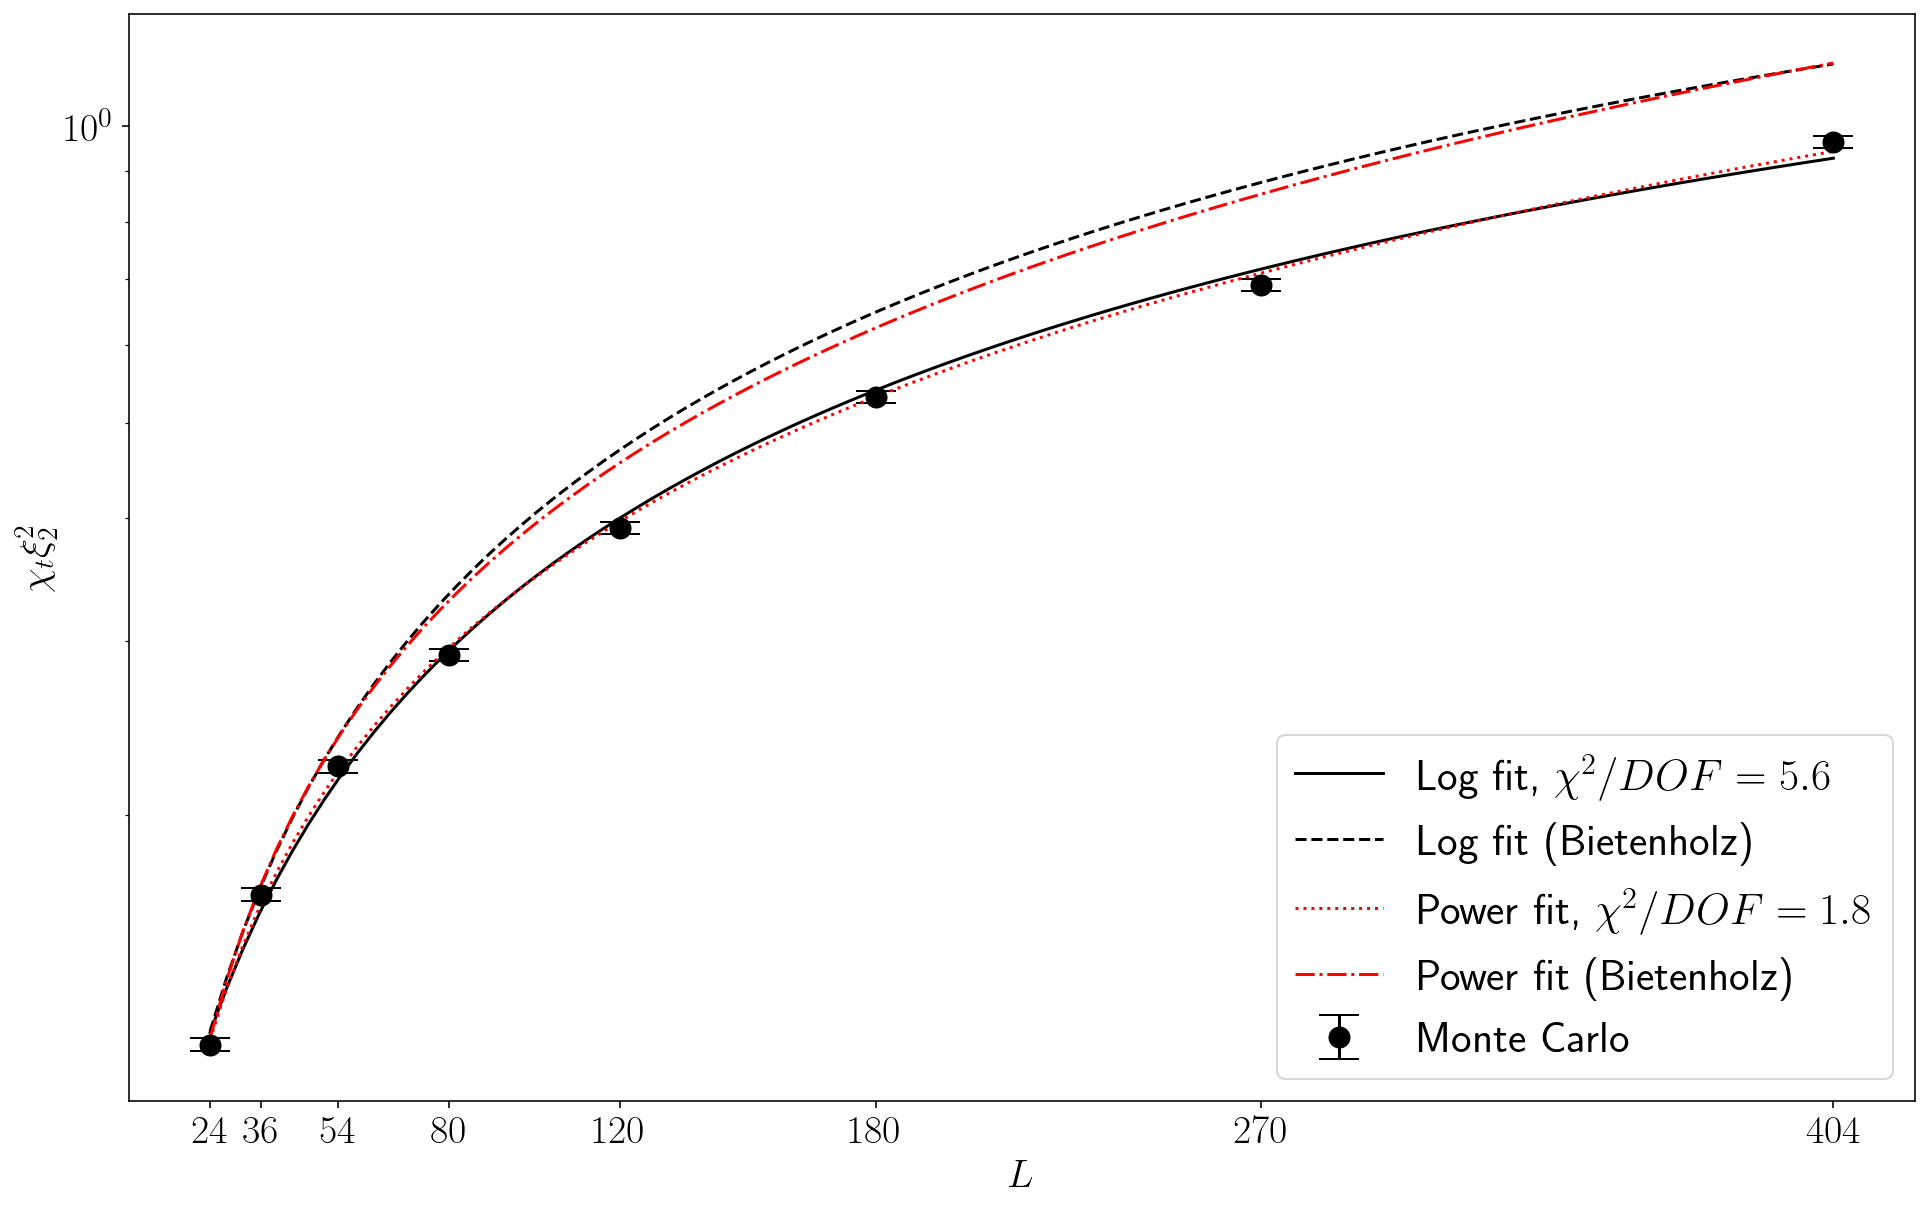
\includegraphics[width=0.9\textwidth]{imgs/divergence.png}
              \caption{$\tau = 0$}
          \end{subfigure}%
          \begin{subfigure}[b]{0.45\paperwidth}
              \centering
              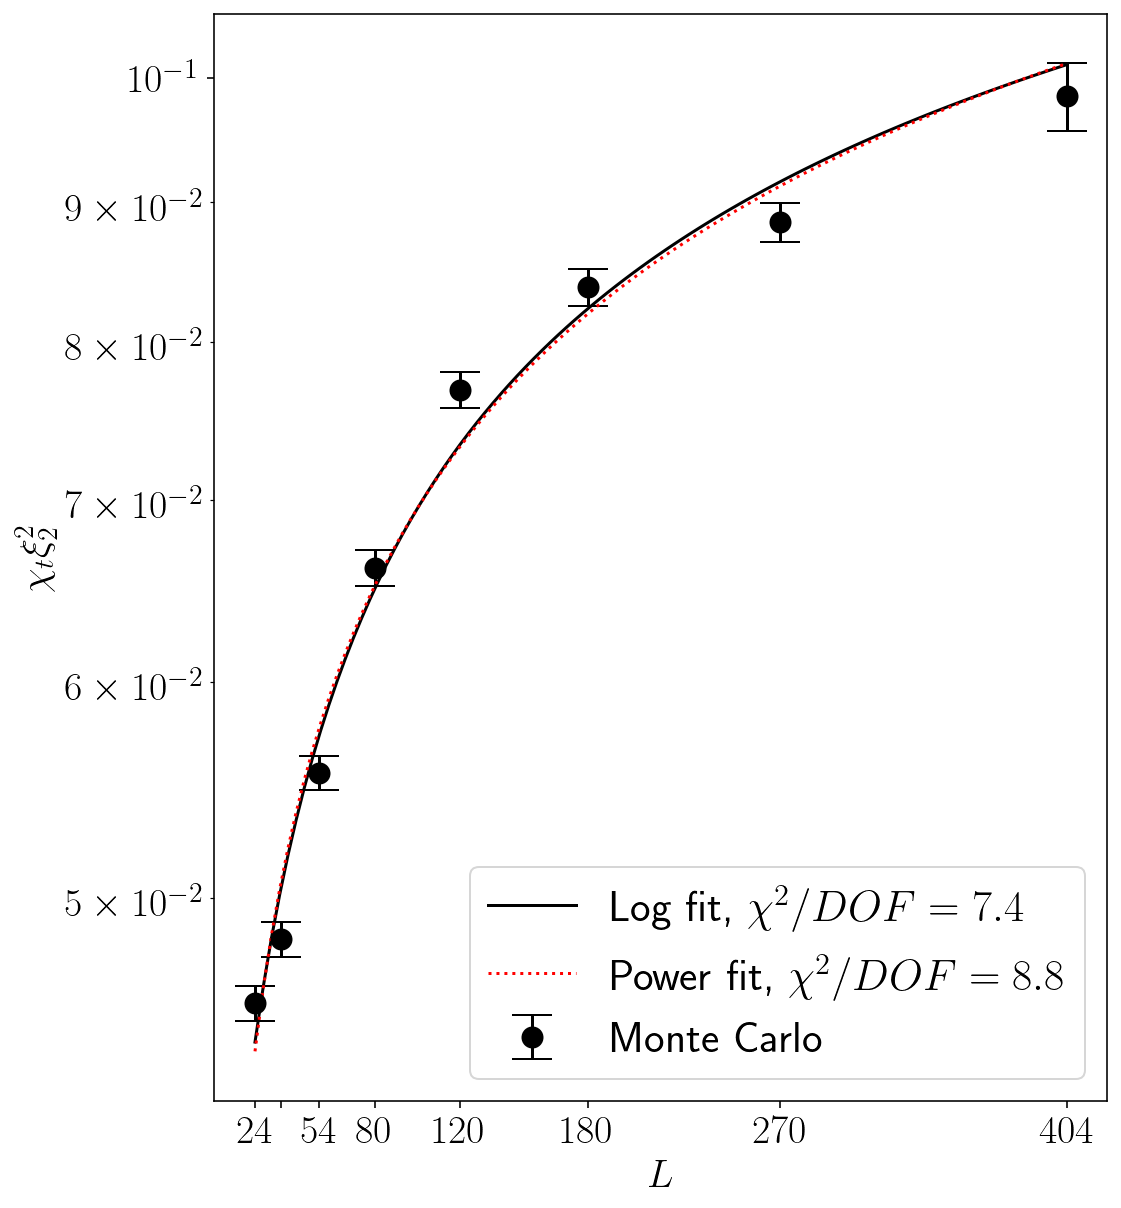
\includegraphics[width=0.9\textwidth]{imgs/divergence_flowed.png}
              \caption{$\tau = 5t_0$}
          \end{subfigure}
        \end{center}
        \caption{Divergent properties with comparison to~\footfullcite{bietenholz2018}, 10,000 measurements}
    \end{figure}
          \note{Simulation run with 10,000 measurements, once every 50 sweeps, 1,000 sweep thermalization. In the tau=0 case, we have compared our result with the curve fit found in Bietenholz}
\end{frame}

\begin{frame}
    \frametitle{Effect of $\theta$-term on $\langle Q \rangle$}
    \begin{figure}[h]
          \centering
          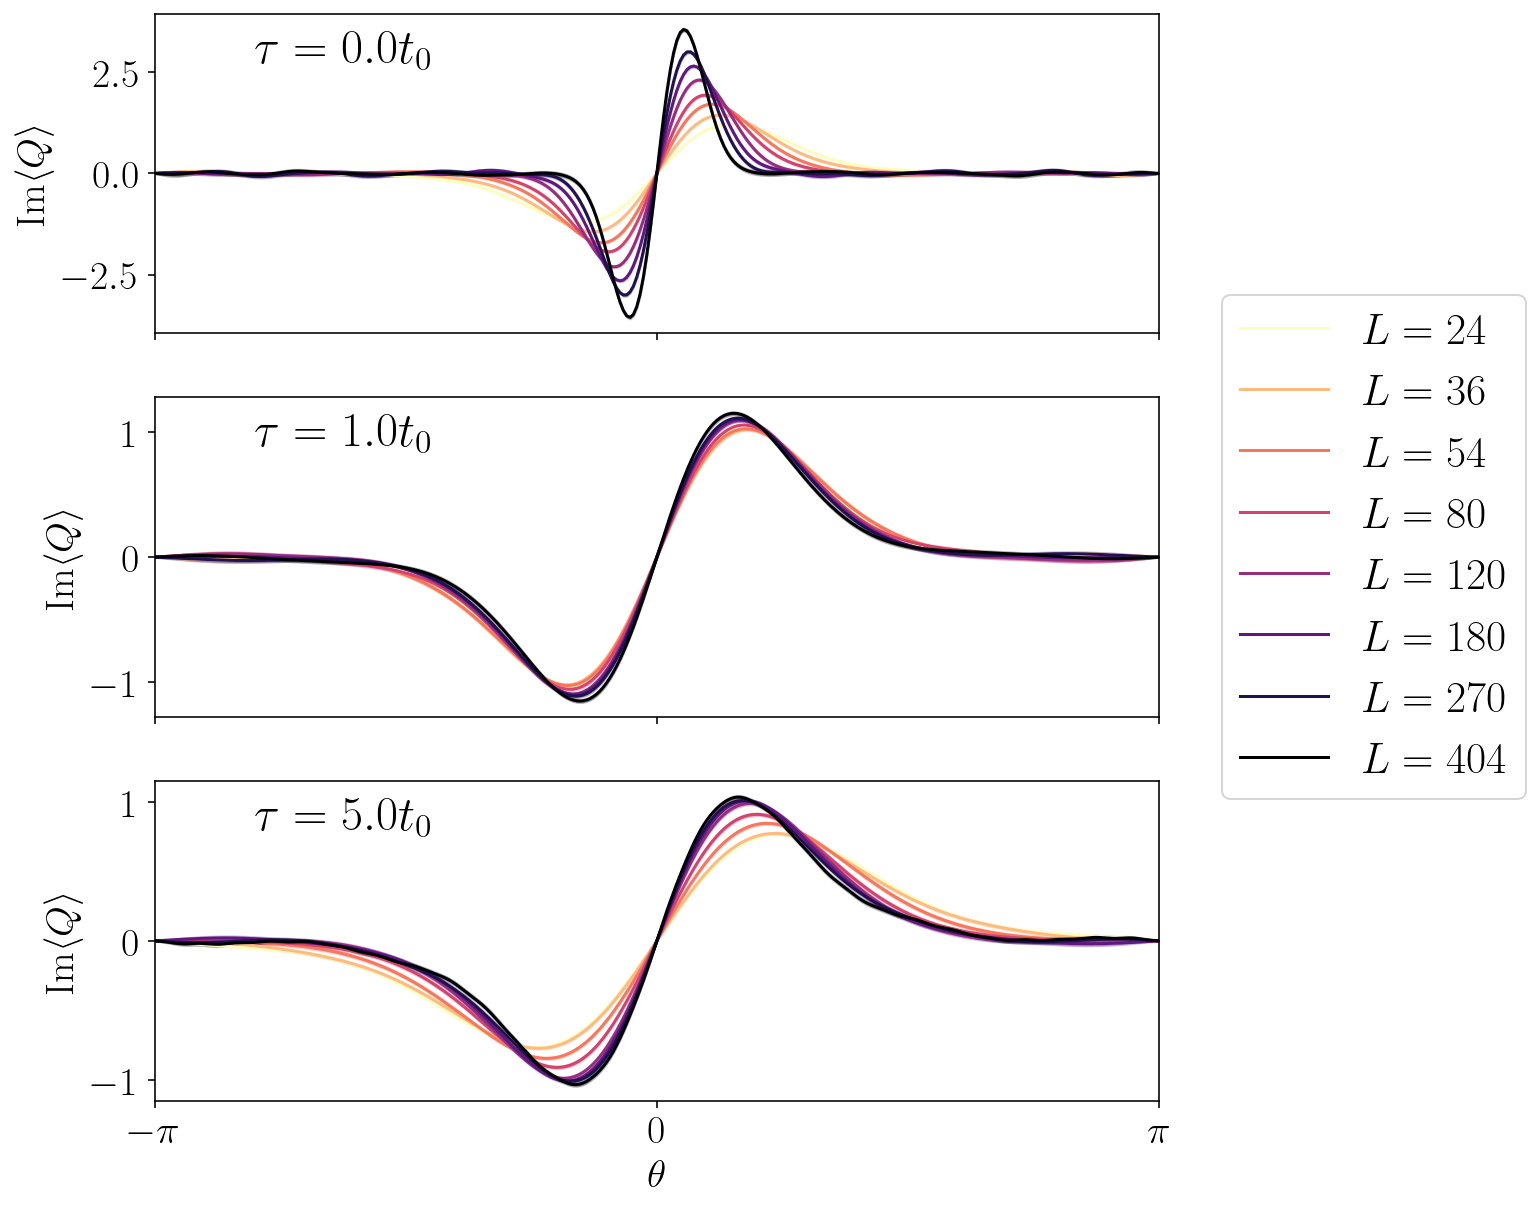
\includegraphics[width=0.8\textwidth]{imgs/theta.png}
    \end{figure}
\end{frame}

\begin{frame}
    \frametitle{Conclusions}
    \begin{itemize}
        \item  Berg \& L\"uscher~\footfullcite{berg1981} provide three possible reasons
            \begin{enumerate}
                \only<1>{\item high-frequency modes cause divergence}
                \only<2->{\item {\transparent{0.4} high-frequency modes cause divergence}}
                \item the definition of $Q$ is problematic
                \item the NLSM has no well-defined continuum limit
            \end{enumerate}

        \item<3-> Relatively high $\chi^2/DOF$ values indicate errors underestimated.
        \item<4-> Clearer perspective on the effect $\theta$ helpful for condensed matter systems~\footfullcite{bogli2012}.
    \end{itemize}
\end{frame}
\begin{frame}
    \frametitle{Acknowledgements}
    \begin{itemize}
        \item<1-> 1693 Scholars program (funding for summer research)
        \item<2-> HPC Computing Group
        \item<3-> Prof. Christopher Monahan
        \item<4-> Friends and family
    \end{itemize}
\end{frame}
\end{document} 

